% =============================================================================
% CAPÍTULO III - METODOLOGÍA
% =============================================================================

\cleardoublepage
\thispagestyle{empty}
\vspace*{\fill}
\begin{center}
{\Large\bfseries CAPÍTULO III}\\[2.5cm]
{\Large\bfseries METODOLOGÍA}
\end{center}
\vspace*{\fill}
\clearpage

\chapter*{}
\addcontentsline{toc}{chapter}{CAPÍTULO III -- METODOLOGÍA}
\setcounter{chapter}{3}
\setcounter{section}{0}
\renewcommand{\thesection}{3.\arabic{section}}
\renewcommand{\thesubsection}{3.\arabic{section}.\arabic{subsection}}

\vspace{-3cm}

\section{Marco de fases de desarrollo del proyecto tecnológico}

El desarrollo del proyecto se dividió en tres etapas principales: la obtención de requisitos, el desarrollo de la aplicación y las pruebas e implementación. Esta distribución se alinea con la propuesta de Braumer \cite{ref55_braumer}, la cual consiste en la presentación de prototipos o incrementos funcionales para la visualización temprana de las interfaces y la evaluación continua de las funcionalidades a lo largo del proyecto. Para ejecutar este flujo de trabajo se aplicaron las prácticas de la Programación Extrema (XP), adaptadas al contexto específico del proyecto. Al tratarse de un desarrollo individual, las prácticas colaborativas de XP se enfocaron en la autodisciplina y la revisión personal, mientras que la evaluación continua con los expertos se estructuró en ciclos de retroalimentación planificados en función de su disponibilidad. De esta manera, la obtención de requisitos se gestionó mediante el Juego de Planificación y la creación de Historias de Usuario; el desarrollo de la aplicación se centró en el ciclo de \textit{Test-Driven Development} (TDD), la refactorización y el diseño simple; y, finalmente, las pruebas e implementación se basaron en la integración continua y la entrega de lanzamientos pequeños para la validación del cliente, según se ilustra en la Ilustración~\ref{fig:metodologia_xp}.

\begin{figure}[H]
\centering
\caption{Metodología XP (Programación Extrema) aplicada al proyecto Kiddy Quiz.}
\label{fig:metodologia_xp}
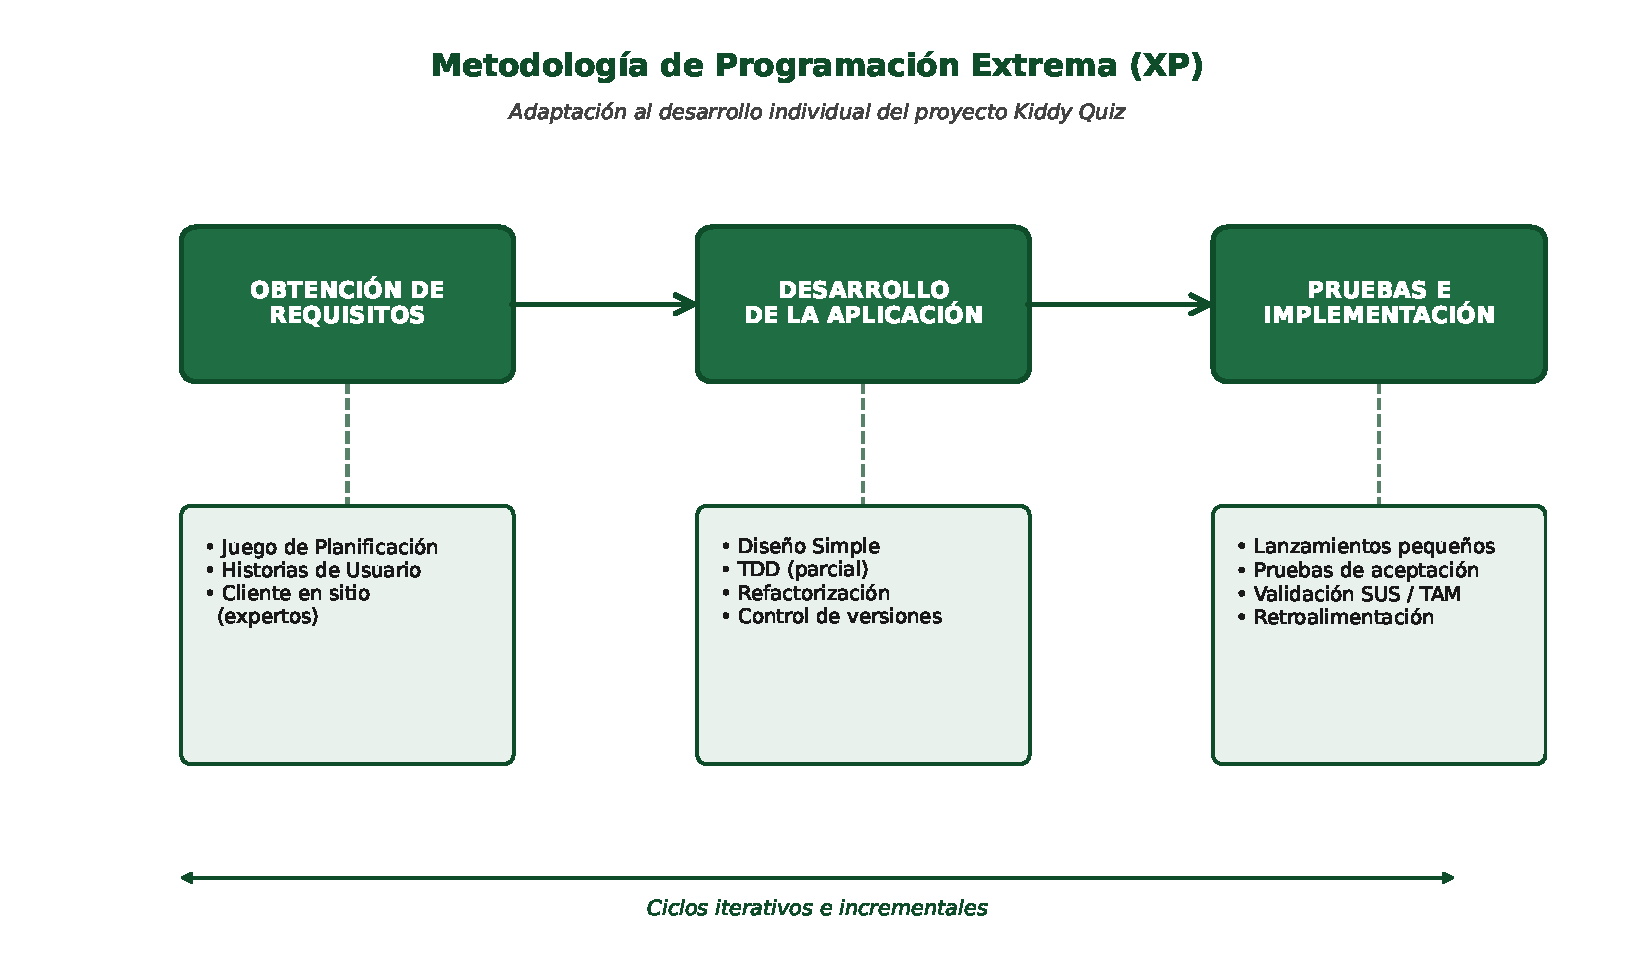
\includegraphics[width=0.95\textwidth]{figuras/fig01_metodologia_xp.pdf}
\fuente{Adaptado de Ganney et al.\ \cite{ref47_ganney_xp}}
\end{figure}

\subsection{Obtención de requisitos}

La fase de obtención de requisitos tuvo como objetivo principal comprender de manera integral las necesidades pedagógicas y cognitivas asociadas a la evaluación por competencias en matemáticas en el nivel de educación básica elemental, superando un enfoque limitado a aspectos exclusivamente técnicos. Para ello, se aplicó el juego de planificación o \textit{Planning Game}, una práctica central de la metodología XP, adaptada al contexto académico y a las características del proyecto.

Dado que el desarrollo se realizó de forma individual, la interacción con los usuarios finales se estructuró a través de ciclos de comunicación planificados con expertos en evaluación por competencias, quienes asumieron el rol de cliente en el sitio o \textit{On-site Customer}. Este enfoque permitió establecer un canal de retroalimentación constante y asegurar que los requerimientos del sistema respondieran a necesidades reales del contexto educativo.

\textbf{Análisis preliminar y contextual.} Como punto de partida se llevó a cabo un análisis preliminar orientado a evaluar la viabilidad del proyecto y a delimitar su alcance funcional. En esta etapa se identificó a los expertos que participarían en el proceso, conformados por cinco docentes de educación básica elemental con experiencia en evaluación por competencias y dos psicopedagogos vinculados al ámbito universitario.

Las entrevistas a los docentes se realizaron de manera presencial y tuvieron un carácter formal, con el propósito de recopilar información detallada sobre sus prácticas evaluativas, los desafíos enfrentados en la enseñanza de matemáticas y las limitaciones de los métodos tradicionales de evaluación. En contraste, las entrevistas a los psicopedagogos se llevaron a cabo en la Universidad Técnica Estatal de Quevedo bajo un enfoque no estructurado, orientado a guiar el diseño pedagógico e inclusivo del sistema desde una perspectiva especializada. Todas las entrevistas fueron individuales. Previo a su ejecución, se obtuvo el consentimiento informado por escrito de los participantes (véase Anexo~A), autorizando el uso académico de la información recopilada.

\textbf{Ejecución del Juego de Planificación.} El Juego de Planificación se aplicó a los docentes mediante entrevistas semiestructuradas apoyadas en una guía de diez preguntas previamente definida (véase Anexo~A). Cada entrevista tuvo una duración aproximada de cuarenta minutos. Las preguntas se enfocaron en cuatro ejes principales: la experiencia docente en la enseñanza de matemáticas, los desafíos asociados a la evaluación de competencias matemáticas, el uso de herramientas digitales en los procesos evaluativos y las expectativas respecto a una aplicación orientada a evaluaciones por competencias. Asimismo, se abordaron aspectos relacionados con los tipos y formatos de preguntas más adecuados, la diversidad de contenidos evaluativos y las funcionalidades necesarias para el análisis y seguimiento de los resultados de los estudiantes.

Durante el desarrollo de las entrevistas se presentaron interfaces preliminares del sistema como prototipos funcionales obtenidos de la revisión de aplicaciones existentes (Kahoot!, Quizizz, Nearpod, Socrative y ClassDojo), lo cual permitió \textit{amplificar el aprendizaje}, una práctica característica de XP. Esta estrategia facilitó la comprensión de los requisitos y promovió una retroalimentación más precisa por parte de los expertos, especialmente en lo referente a la usabilidad y al diseño orientado a estudiantes de educación básica.

\textbf{Definición y documentación de Historias de Usuario.} A partir de la información recopilada se procedió a la definición y documentación de las historias de usuario, las cuales constituyeron el principal insumo para la planificación del desarrollo del sistema. En total se elaboraron veintinueve historias de usuario, redactadas desde una perspectiva centrada principalmente en el rol del docente como usuario responsable de la gestión de evaluaciones y del seguimiento del progreso académico de los estudiantes.

Cada historia de usuario incluyó criterios de aceptación de carácter pedagógico, definidos en conjunto con los expertos, los cuales orientaron la validación de las funcionalidades desarrolladas. Entre los criterios más relevantes se destacan la necesidad de un diseño intuitivo y visualmente atractivo para los estudiantes, la incorporación de formatos de preguntas variados y la disponibilidad de herramientas que permitan un seguimiento detallado de los resultados de las evaluaciones. La priorización de las historias de usuario permitió organizar el trabajo en incrementos funcionales, sentando las bases para la fase de desarrollo y asegurando la entrega progresiva de valor conforme a los principios de la metodología XP.

\subsection{Desarrollo de la aplicación}

La fase de desarrollo de la aplicación constituyó el núcleo del proyecto, etapa en la cual se materializaron los requerimientos definidos durante la primera fase. Se ejecutó siguiendo los principios de la metodología XP, priorizando ciclos de desarrollo cortos, la simplicidad en el diseño y la entrega continua de funcionalidades operativas. El desarrollo se llevó a cabo de manera individual, lo que implicó una adaptación consciente de ciertas prácticas colaborativas de XP, manteniendo el rigor técnico y la disciplina metodológica.

Dado el carácter individual del desarrollo, la práctica de \textit{Pair Programming} se adaptó a un enfoque de autoevaluación y revisión crítica del código. Para ello se destinó tiempo específico a la revisión sistemática de las funcionalidades implementadas y se aplicó la técnica del \textit{patito de goma}, la cual consiste en explicar en voz alta la lógica del código desarrollado. Adicionalmente, de manera ocasional, el código fue presentado al director del proyecto para su revisión y retroalimentación, lo que permitió identificar inconsistencias, errores lógicos y oportunidades de mejora. El control de versiones del proyecto se gestionó mediante GitHub, lo que facilitó el seguimiento de los cambios realizados, la organización del código fuente y la estabilidad del sistema durante su evolución.

\textbf{Generación y adaptación de modelos.} Desde la perspectiva del docente se implementaron funcionalidades orientadas a la gestión de clases, evaluaciones y preguntas, la administración de estudiantes y la generación de reportes, permitiéndole planificar, supervisar y analizar el proceso de evaluación. Posteriormente, desde la perspectiva del estudiante, el sistema permite el acceso a las clases y evaluaciones asignadas, la visualización de su progreso académico y la participación en actividades de refuerzo, asegurando una separación clara de responsabilidades entre los distintos roles del sistema.

Durante el desarrollo se priorizó el principio de diseño simple, evitando un modelado exhaustivo previo y permitiendo que la estructura del sistema evolucionara de acuerdo con las necesidades reales del proyecto. Los modelos conceptuales y diagramas se elaboraron únicamente en casos puntuales, como la definición de la arquitectura general del sistema, la comprensión de la interacción entre módulos críticos y la clarificación de flujos complejos de evaluación y seguimiento, antes de iniciar su implementación.

\textbf{Generación de pruebas y software (Desarrollo Dirigido por Pruebas).} La implementación del software se realizó aplicando de manera parcial el enfoque de \textit{Test-Driven Development} (TDD), como una adaptación de la metodología XP, debido principalmente al tiempo limitado del proyecto y a la complejidad de ciertos componentes. Esta aplicación combinó criterios técnicos y metodológicos, permitiendo priorizar la estabilidad del sistema sin afectar el avance progresivo de las funcionalidades. En los módulos críticos del sistema --específicamente en la gestión de clases y en el cálculo de resultados y seguimiento del progreso académico-- se siguió el ciclo característico de TDD: inicialmente se definieron pruebas automatizadas que fallaban, posteriormente se implementó el código mínimo necesario para superarlas y, finalmente, se realizaron procesos de refactorización orientados a mejorar la calidad del código.

Las pruebas desarrolladas incluyeron pruebas unitarias y de integración, enfocadas principalmente en los servicios y en la validación de la interacción entre el \textit{frontend} y el \textit{backend} del sistema. Para su ejecución se empleó el framework Jest, integrado al entorno de desarrollo Visual Studio Code, en un proyecto construido con NestJS para el \textit{backend} y Angular para el \textit{frontend}, utilizando Node.js como entorno de ejecución, npm como gestor de dependencias, GitHub como sistema de control de versiones y PostgreSQL como sistema de gestión de base de datos.

\textbf{Refactorización continua del código.} La refactorización se aplicó como una práctica constante a lo largo de los ciclos de desarrollo, orientada a mejorar la legibilidad, estructura y mantenibilidad del código sin alterar su comportamiento funcional. Esta actividad permitió reducir la complejidad de los módulos implementados, eliminar duplicación de código y adaptar la arquitectura del sistema a medida que se incorporaban nuevas funcionalidades, en concordancia con los principios de XP.

\subsection{Pruebas e implementación}

La fase de pruebas e implementación se orientó a la validación progresiva del sistema y a la verificación de que las funcionalidades desarrolladas respondieran a los requisitos definidos durante la fase de planificación. En concordancia con los principios de XP, esta etapa se centró en la evaluación continua del software mediante incrementos funcionales, aun cuando ciertas prácticas, como la integración continua automatizada, fueron adaptadas a las condiciones reales del proyecto.

\textbf{Refinamiento del software.} El refinamiento del software se llevó a cabo de manera constante a lo largo del proceso de desarrollo, mediante actividades de refactorización orientadas a mejorar la estructura interna del código sin modificar su comportamiento funcional. Esta práctica permitió optimizar la legibilidad, reducir la complejidad de los módulos implementados y facilitar la incorporación de ajustes derivados de las pruebas funcionales y de usabilidad.

\textbf{Implementación del software.} La implementación se gestionó mediante un repositorio de control de versiones alojado en GitHub, que permitió organizar el código fuente, registrar los cambios realizados y mantener un historial claro de las versiones desarrolladas. El desarrollo se realizó de manera iterativa, abordando inicialmente la implementación del \textit{backend} y del \textit{frontend} y trabajando de forma paralela durante las etapas de corrección y ajuste. En una primera fase se estableció la estructura base del sistema, definiendo la arquitectura general, el modelo de base de datos y los módulos relacionados con la autenticación, la gestión de usuarios, las evaluaciones y los reportes. Posteriormente, en el \textit{frontend} se priorizó la implementación completa del flujo de evaluación desde la perspectiva del estudiante.

\textbf{Evaluación del entregable.} La evaluación de los entregables se realizó de manera iterativa, considerando tanto pruebas de funcionamiento como pruebas de usabilidad. Las pruebas funcionales se orientaron a verificar el correcto cumplimiento de los requerimientos definidos. Paralelamente, con la participación de cinco docentes de educación básica elemental, se llevaron a cabo pruebas de usabilidad mediante observación directa y la aplicación de instrumentos estandarizados, específicamente la \textit{System Usability Scale} (SUS) y el \textit{Technology Acceptance Model} (TAM). Estas pruebas permitieron analizar la interacción de los usuarios con la aplicación, identificar dificultades en la navegación y evaluar la claridad de las interfaces.

\textbf{Pruebas de aceptación.} Las pruebas de aceptación constituyeron la etapa final de validación del sistema, orientada a verificar que el software desarrollado cumpliera con las expectativas y necesidades de los expertos en evaluación por competencias. Si bien no se estableció un proceso formal de validación continua con los docentes durante cada incremento, la aprobación previa de módulos individuales como resultado de la evaluación de los criterios de aceptación facilitó la evaluación de la integración final del sistema. La retroalimentación obtenida confirmó la pertinencia del enfoque adoptado, destacándose el diseño intuitivo de la aplicación, la claridad en la presentación de las evaluaciones y la utilidad de las herramientas de seguimiento del progreso académico.

\subsection{Evaluación de la aplicación}

La evaluación de la aplicación tuvo como objetivo analizar su funcionamiento, usabilidad y aceptación desde la perspectiva de los usuarios finales, considerando tanto a estudiantes de educación básica elemental como a docentes expertos en evaluación por competencias. Esta fase se llevó a cabo una vez finalizado el desarrollo del sistema, con el propósito de obtener evidencia empírica que permitiera valorar el cumplimiento de los objetivos planteados.

El proceso de evaluación se realizó con la participación de quince estudiantes de educación básica elemental y cinco docentes con experiencia en evaluaciones por competencias. La evaluación no se desarrolló en el marco de una institución educativa específica, sino mediante sesiones controladas en las que los participantes interactuaron directamente con la aplicación. Para la recolección de información se emplearon diversos instrumentos: una rúbrica de observación, apuntes de campo y los cuestionarios estandarizados SUS (versión castellana) y TAM (versión castellana), disponibles en los Anexos~B y~C. Estos instrumentos permitieron obtener tanto datos cualitativos como cuantitativos, orientados a medir aspectos relacionados con la eficiencia, efectividad y satisfacción de los usuarios.

\section{Cronograma}

Para alcanzar los objetivos del proyecto, en la Ilustración~\ref{fig:cronograma} se presenta un cronograma de treinta y dos semanas que detalla las actividades realizadas a lo largo del proceso de desarrollo. Estas abarcan desde el análisis y la estructuración del tema hasta la entrega de la documentación correspondiente al trabajo de integración curricular.

\begin{figure}[H]
\centering
\caption{Cronograma de actividades del proyecto Kiddy Quiz.}
\label{fig:cronograma}
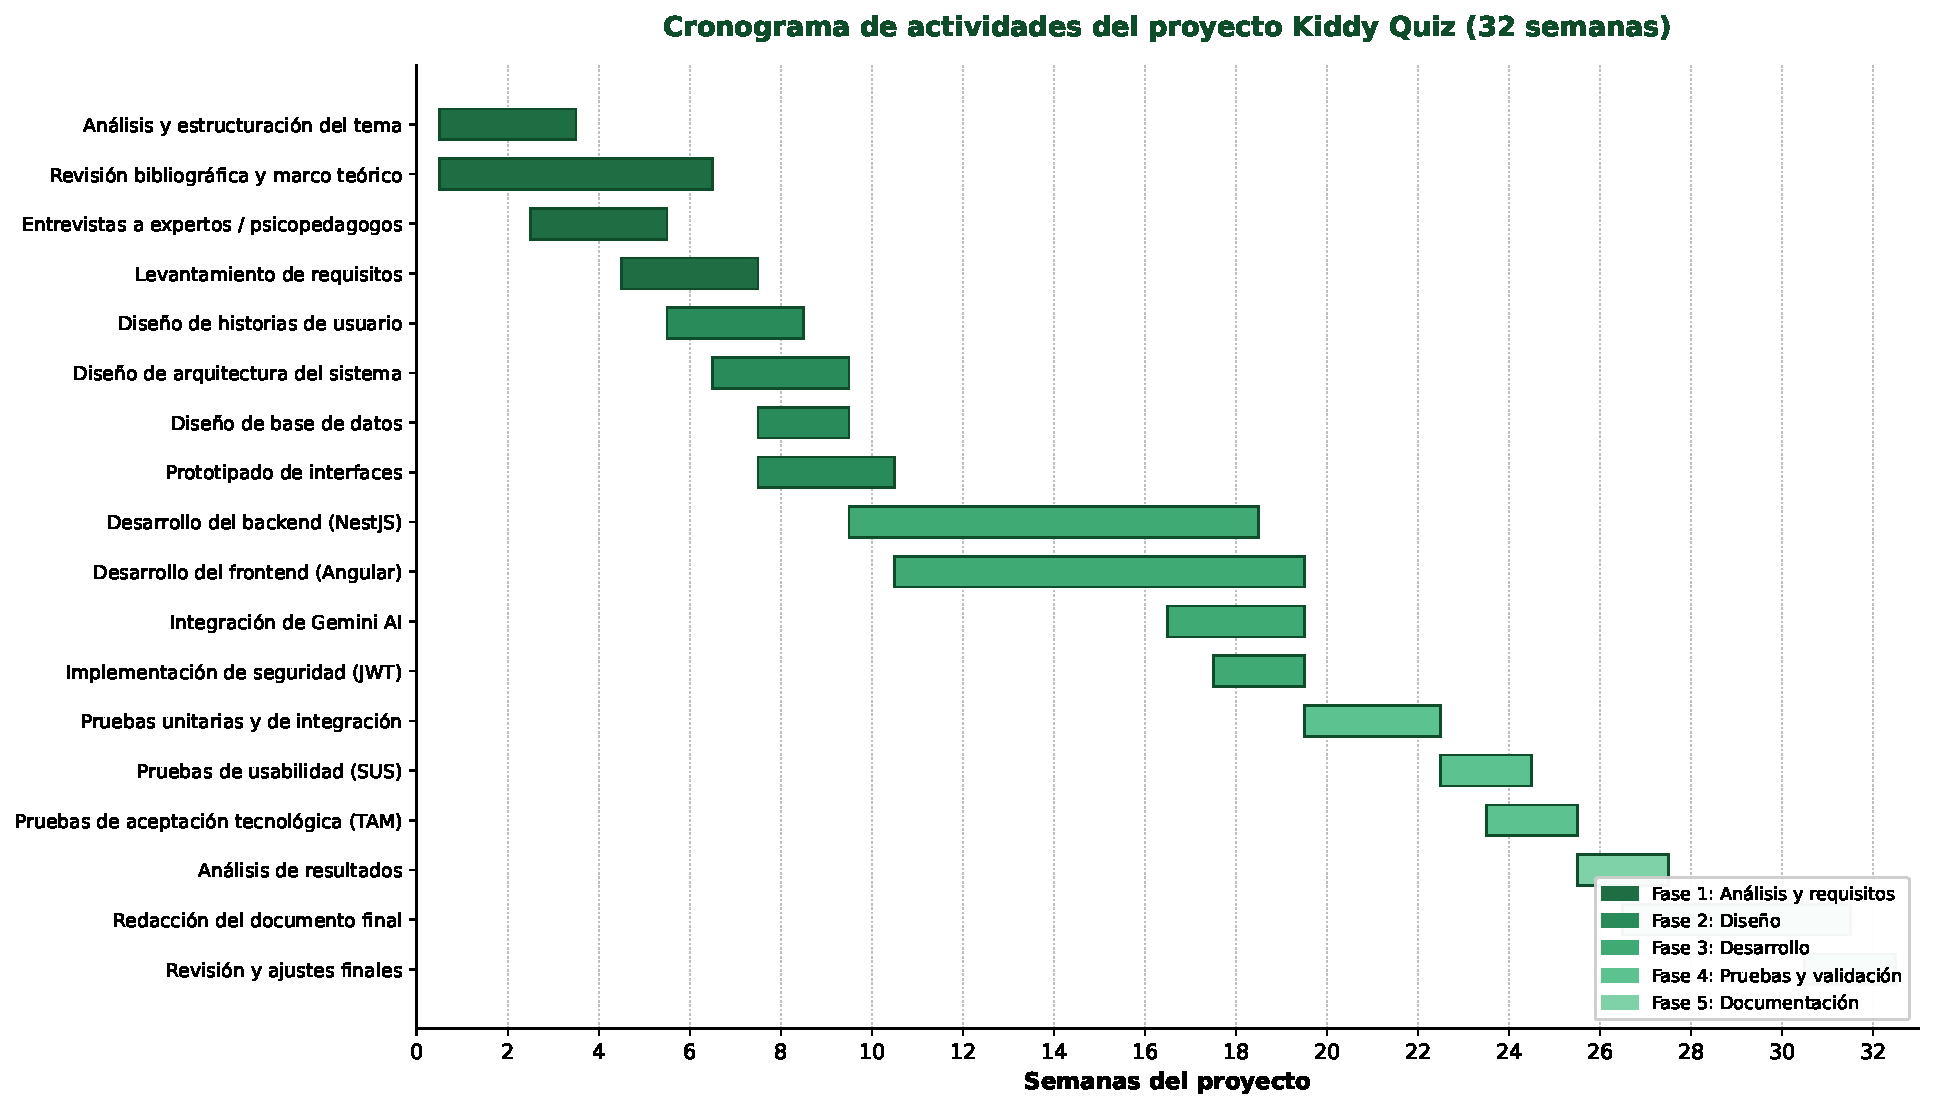
\includegraphics[width=\textwidth]{figuras/fig02_cronograma.pdf}
\fuenteautor
\end{figure}

\section{Recursos, presupuesto y financiamiento}

En la Tabla~\ref{tab:presupuesto} se presenta el presupuesto que cubre los recursos para el desarrollo de Kiddy Quiz. Se detallan los insumos y herramientas utilizadas, incluyendo dispositivos electrónicos, materiales de oficina y servicios en la nube necesarios para el almacenamiento y procesamiento de datos. El costo total se compone de inversiones únicas en hardware y software utilizados en el proyecto, asumidas íntegramente por el autor.

\begin{table}[H]
\centering
\caption{Presupuesto del proyecto Kiddy Quiz.}
\label{tab:presupuesto}
\begin{small}
\begin{tabularx}{\textwidth}{|L{2.7cm}|L{3.0cm}|X|R{1.6cm}|R{1.5cm}|}
\hline
\rowcolor{tabhead}
\tabhead{Categoría} & \tabhead{Concepto} & \tabhead{Descripción} & \tabhead{Aporta} & \tabhead{Costo (USD)}\\
\hline
Materiales e insumos & Computadora portátil & Equipo principal de desarrollo (Intel i5, 16~GB RAM) & Personal & 800.00\\
\hline
 & Mouse y teclado & Periféricos para entrevistas y desarrollo & Personal & 35.00\\
\hline
 & Suministros de oficina & Hojas, esferográficos para entrevistas & Personal & 20.00\\
\hline
Servicios & Conexión a Internet & Servicio mensual durante 8 meses & Personal & 240.00\\
\hline
 & Energía eléctrica & Consumo durante el desarrollo & Personal & 80.00\\
\hline
 & Movilización & Traslado a entrevistas con expertos & Personal & 60.00\\
\hline
Tecnologías de desarrollo & Visual Studio Code & Editor de código fuente (gratuito) & Microsoft & 0.00\\
\hline
 & Angular, NestJS, Node.js & \textit{Frameworks} y entorno de ejecución (\textit{open source}) & Comunidad & 0.00\\
\hline
 & PostgreSQL & Sistema de base de datos relacional (\textit{open source}) & PGDG & 0.00\\
\hline
 & GitHub (cuenta gratuita) & Repositorio de control de versiones & GitHub Inc. & 0.00\\
\hline
 & Gemini API (capa gratuita) & Modelo de IA generativa & Google & 0.00\\
\hline
Recursos humanos & Profesionales en educación & Cinco docentes y dos psicopedagogos & Universidad / Voluntario & 0.00\\
\hline
Imprevistos (10\,\%) &  &  & Personal & 124.00\\
\hline
\rowcolor{tabhead2}
\multicolumn{4}{|r|}{\textbf{TOTAL}} & \textbf{1\,359.00}\\
\hline
\end{tabularx}
\end{small}
\fuenteautor
\end{table}

\section{Instrumentos para el seguimiento y control}

El seguimiento y control del proyecto se constituyeron como actividades fundamentales para garantizar el cumplimiento de los objetivos planteados, el uso adecuado de los recursos disponibles y el desarrollo ordenado de las fases definidas en la metodología. Para ello se emplearon diversos instrumentos y herramientas tecnológicas que permitieron planificar las actividades, monitorear el avance del proyecto, gestionar la documentación y controlar la evolución del software desarrollado.

En cuanto a la gestión y seguimiento de tareas, se utilizó Microsoft Excel como herramienta principal de planificación. A través de esta aplicación se estructuró una tabla de control en la que las actividades del proyecto fueron organizadas en tres estados (pendiente, en proceso y completado), facilitando la visualización del progreso y permitiendo realizar ajustes oportunos. Asimismo, se elaboró un diagrama de Gantt y una lista detallada de actividades en Excel, lo que permitió establecer tiempos estimados de inicio y finalización.

El control de versiones del software se llevó a cabo mediante GitHub, utilizando un repositorio público que permitió gestionar de forma ordenada los cambios realizados en el código fuente. Durante el desarrollo se emplearon dos ramas de trabajo, debido a que el proyecto fue desarrollado desde dos computadoras con sistemas operativos distintos (Windows y macOS). Esta estrategia facilitó la integración del código, la sincronización de los avances y la recuperación de versiones anteriores en caso de ser necesario.

Para la gestión de la documentación se utilizaron de manera complementaria el almacenamiento local y Google Drive. En estos espacios se organizaron los documentos relacionados con las entrevistas, los formatos de consentimiento informado, los anexos, las capturas de las interfaces del sistema y la documentación técnica generada. La comunicación y retroalimentación con los docentes expertos se realizó principalmente de manera presencial y a través de WhatsApp, lo que permitió una interacción ágil y espontánea.

En lo referente al seguimiento técnico y la validación del software, se implementaron pruebas automatizadas utilizando el framework Jest. Estas pruebas permitieron verificar el correcto funcionamiento de distintos componentes del sistema, así como detectar errores asociados a determinados \textit{endpoints}, especialmente los relacionados con el seguimiento del progreso del estudiante y la retroalimentación generada por el módulo de inteligencia artificial. Para la elaboración de la documentación formal, el análisis de información y la presentación de resultados se emplearon herramientas ofimáticas de Microsoft Office: Word para la redacción del documento, Excel para tablas, cronogramas y registros, y PowerPoint para presentaciones.

Finalmente, en cuanto a la gestión de riesgos, se identificaron diversos factores que podrían afectar el desarrollo del proyecto, tales como limitaciones de tiempo, disponibilidad de los expertos, complejidad técnica del sistema y posibles dificultades en la implementación de determinadas funcionalidades. Estos riesgos se gestionaron a través de la reorganización de tareas y el ajuste de la planificación.

\section{Indicadores de evaluación}

En esta sección se describen los indicadores de evaluación utilizados para verificar el cumplimiento de las especificaciones del proyecto tecnológico, así como para analizar de manera crítica los resultados obtenidos durante su desarrollo. Estos indicadores permitieron validar que el sistema responde al problema planteado, cumple con los requisitos definidos y satisface las necesidades de los usuarios finales.

Las actividades de verificación y validación se ejecutaron a lo largo de las distintas fases del proyecto, considerando aspectos relacionados con el cumplimiento del cronograma, el alcance funcional, la calidad del sistema, la usabilidad, la aceptación tecnológica, el rendimiento técnico, la seguridad básica y el nivel de innovación educativa. Los indicadores se presentan en las Tablas~\ref{tab:ind_plazos} a~\ref{tab:ind_innovacion}.

\begin{table}[H]
\centering
\caption{Indicador de cumplimiento de plazos.}
\label{tab:ind_plazos}
\begin{tabularx}{\textwidth}{|L{3.5cm}|X|}
\hline
\rowcolor{tabhead}
\tabhead{Indicador} & \tabhead{Cumplimiento de plazos}\\
\hline
\textbf{Descripción} & Mide la capacidad del proyecto para cumplir con los tiempos establecidos para el desarrollo de las actividades y fases definidas en el cronograma.\\
\hline
\textbf{Medición} & Se estableció un cronograma inicial que fue ajustado durante el desarrollo. Se utilizaron diagramas de Gantt y listas de tareas en Microsoft Excel, organizadas en estados ``Pendiente'', ``En proceso'' y ``Completado''. Se compararon las fechas planificadas con las fechas reales.\\
\hline
\textbf{Criterios de éxito} & Se considera satisfactorio el cumplimiento si al menos el 90\,\% de las tareas fueron completadas dentro de los plazos ajustados, aceptando retrasos leves no críticos.\\
\hline
\end{tabularx}
\fuenteautor
\end{table}

\begin{table}[H]
\centering
\caption{Indicador de cumplimiento del alcance del proyecto.}
\label{tab:ind_alcance}
\begin{tabularx}{\textwidth}{|L{3.5cm}|X|}
\hline
\rowcolor{tabhead}
\tabhead{Indicador} & \tabhead{Cumplimiento del alcance}\\
\hline
\textbf{Descripción} & Evalúa el grado de cumplimiento de los objetivos y requisitos funcionales definidos para el sistema.\\
\hline
\textbf{Medición} & Se verificó la implementación de las veintinueve historias de usuario definidas durante la fase de análisis. Se realizó una validación funcional de los módulos principales del sistema.\\
\hline
\textbf{Criterios de éxito} & Se considera satisfactorio si todas las historias de usuario fueron implementadas y las funcionalidades principales operan correctamente.\\
\hline
\end{tabularx}
\fuenteautor
\end{table}

\begin{table}[H]
\centering
\caption{Indicador de calidad del producto.}
\label{tab:ind_calidad}
\begin{tabularx}{\textwidth}{|L{3.5cm}|X|}
\hline
\rowcolor{tabhead}
\tabhead{Indicador} & \tabhead{Calidad del sistema}\\
\hline
\textbf{Descripción} & Mide el nivel de calidad del sistema en términos de estabilidad, funcionalidad y ausencia de errores críticos.\\
\hline
\textbf{Medición} & Se realizaron pruebas unitarias, pruebas de integración y pruebas funcionales manuales, ejecutadas de forma parcial antes de la evaluación con usuarios.\\
\hline
\textbf{Criterios de éxito} & Se considera de calidad adecuada si no se presentan errores críticos que afecten su funcionamiento principal.\\
\hline
\end{tabularx}
\fuenteautor
\end{table}

\begin{table}[H]
\centering
\caption{Indicador de usabilidad y satisfacción del usuario.}
\label{tab:ind_usabilidad}
\begin{tabularx}{\textwidth}{|L{3.5cm}|X|}
\hline
\rowcolor{tabhead}
\tabhead{Indicador} & \tabhead{Nivel de satisfacción del usuario}\\
\hline
\textbf{Descripción} & Evalúa la percepción de los usuarios finales sobre la facilidad de uso y la experiencia general del sistema.\\
\hline
\textbf{Medición} & Se aplicó el cuestionario SUS a docentes y estudiantes de educación básica elemental. Se recopiló retroalimentación cualitativa durante las sesiones.\\
\hline
\textbf{Criterios de éxito} & Se considera satisfactorio si la puntuación SUS alcanza o supera el valor de referencia de 68.\\
\hline
\end{tabularx}
\fuenteautor
\end{table}

\begin{table}[H]
\centering
\caption{Indicador de aceptación tecnológica (TAM).}
\label{tab:ind_tam}
\begin{tabularx}{\textwidth}{|L{3.5cm}|X|}
\hline
\rowcolor{tabhead}
\tabhead{Indicador} & \tabhead{Aceptación tecnológica}\\
\hline
\textbf{Descripción} & Mide el nivel de aceptación del sistema por parte de los usuarios, considerando su utilidad y facilidad de uso.\\
\hline
\textbf{Medición} & Se aplicó el modelo TAM evaluando las dimensiones de Facilidad de Uso Percibida (PEOU), Utilidad Percibida (PU) e Intención de Uso (IU).\\
\hline
\textbf{Criterios de éxito} & Se considera aceptado si los usuarios manifiestan percepciones positivas (media superior a 3,5 sobre 5) en las dimensiones evaluadas.\\
\hline
\end{tabularx}
\fuenteautor
\end{table}

\begin{table}[H]
\centering
\caption{Indicador de rendimiento del sistema.}
\label{tab:ind_rendimiento}
\begin{tabularx}{\textwidth}{|L{3.5cm}|X|}
\hline
\rowcolor{tabhead}
\tabhead{Indicador} & \tabhead{Rendimiento técnico}\\
\hline
\textbf{Descripción} & Evalúa el desempeño técnico del sistema durante su uso, considerando estabilidad y tiempos de respuesta.\\
\hline
\textbf{Medición} & Se evaluó el comportamiento del sistema en condiciones de carga y tiempo de respuesta. Se verificó la estabilidad durante las pruebas con usuarios.\\
\hline
\textbf{Criterios de éxito} & Se considera adecuado si el sistema no presenta caídas significativas y mantiene tiempos de respuesta aceptables (inferiores a 2~segundos en operaciones comunes).\\
\hline
\end{tabularx}
\fuenteautor
\end{table}

\begin{table}[H]
\centering
\caption{Indicador de seguridad básica del sistema.}
\label{tab:ind_seguridad}
\begin{tabularx}{\textwidth}{|L{3.5cm}|X|}
\hline
\rowcolor{tabhead}
\tabhead{Indicador} & \tabhead{Seguridad de acceso}\\
\hline
\textbf{Descripción} & Mide la efectividad de los mecanismos básicos de seguridad implementados en el sistema.\\
\hline
\textbf{Medición} & Se verificó la existencia de autenticación mediante inicio de sesión con tokens JWT. Se validó el control de acceso según roles (docente y estudiante).\\
\hline
\textbf{Criterios de éxito} & Se considera satisfactorio si el acceso al sistema está restringido por roles y no se detectaron vulnerabilidades durante el desarrollo.\\
\hline
\end{tabularx}
\fuenteautor
\end{table}

\begin{table}[H]
\centering
\caption{Indicador de innovación y aporte educativo.}
\label{tab:ind_innovacion}
\begin{tabularx}{\textwidth}{|L{3.5cm}|X|}
\hline
\rowcolor{tabhead}
\tabhead{Indicador} & \tabhead{Innovación educativa}\\
\hline
\textbf{Descripción} & Evalúa el nivel de innovación introducido por el proyecto en el contexto educativo.\\
\hline
\textbf{Medición} & Se analizó la incorporación de inteligencia artificial generativa para la retroalimentación académica. Se evaluó el uso de pictogramas para la evaluación por competencias. Se consideró el seguimiento del progreso del estudiante como aporte pedagógico.\\
\hline
\textbf{Criterios de éxito} & Se considera innovador si introduce enfoques y funcionalidades no existentes en el contexto local de la educación básica elemental.\\
\hline
\end{tabularx}
\fuenteautor
\end{table}
